\documentclass[a4,10pt]{article} \usepackage[pdftex]{graphicx}
\usepackage{setspace}
%\usepackage{lineno}
\usepackage{color}
\definecolor{PiranaOrange}{rgb}{0.9,0.4,0.1}
\definecolor{Blue}{rgb}{0.0,0.0,0.7}
\definecolor{Red}{rgb}{0.7,0.0,0.0}
\definecolor{Grey}{rgb}{0.2,0.2,0.2}
\definecolor{grey2}{rgb}{.92, .92, .92}


\pdfinfo{
   /Author (Ron Keizer, Coen van Hasselt, Pirana Software & Consulting BV)
   /Title  (Pirana Quick Guide)
}


\bibliographystyle{unsrt}%Choose a bibliograhpic style}
%\usepackage{utopia} %\usepackage{charter} %\usepackage{palatino}
%\usepackage{bookman} %\usepackage{newcent} %\usepackage{times}
%\usepackage[options]{natbib} \sloppy
\renewcommand{\familydefault}{\sfdefault} 
\renewcommand{\emph}[1]{\textbf{\textcolor{Grey}{#1}}} 
\oddsidemargin 1cm
\textwidth 14cm
\textheight 20cm

\begin{document}

{\centering
  \vspace{-100pt}
  \textbf{
    \textcolor{PiranaOrange}{\Large Pirana}
  }\\
  \vspace{5pt} \scriptsize \textcolor{Grey}{The flexible modeling
    environment for NONMEM} \\ \normalsize
  \vspace{12pt}
  \hspace{5pt}
\includegraphics[scale=0.14]{images/pirana_logo.jpg}\\
  \vspace{18pt}

  {\large
    \emph{Quick Guide: Configuration of Pirana }  \vspace{10pt} \\
        Version 1.1
  }

}
\vspace{25pt}


\begin{center}
   {\colorbox{grey2}{
         \begin{minipage}[t]{0.9\textwidth}
\subsubsection*{Scope}
This Pirana Quick Guide explains how to configure the most important settings in Pirana. 
          \end{minipage}
      }
   }
\end{center}

Most of the settings for Pirana can be configured through the menu File $\rightarrow$ Settings. The following sections deal with the different sections of the Settings window.

\subsubsection*{General settings}
\begin{itemize}
\item The general settings window (Figure 1) deals with some of the general settings for working with Pirana.
\item Most of settings do not need altering to work with Pirana. The meaning of most important settings is discussed below:
\subitem \emph{Alternative data directory}: Alternative location for model input data files.
\subitem \emph{Enable nmfe runs}: If this option is selected, models can be run directly using nmfe.
\subitem \emph{Enable Pirana as wrapper for PsN/WFN/Monolix}: If these options are selected, Pirana may be used to run models through PsN or WFN. Monolix support is experimental.
\subitem \emph{Enable the use of PCluster}: Experimental feature, not supported (refer to PC cluster manual).
\end{itemize}


%% Fig 1 
\begin{figure}[h] \centering
    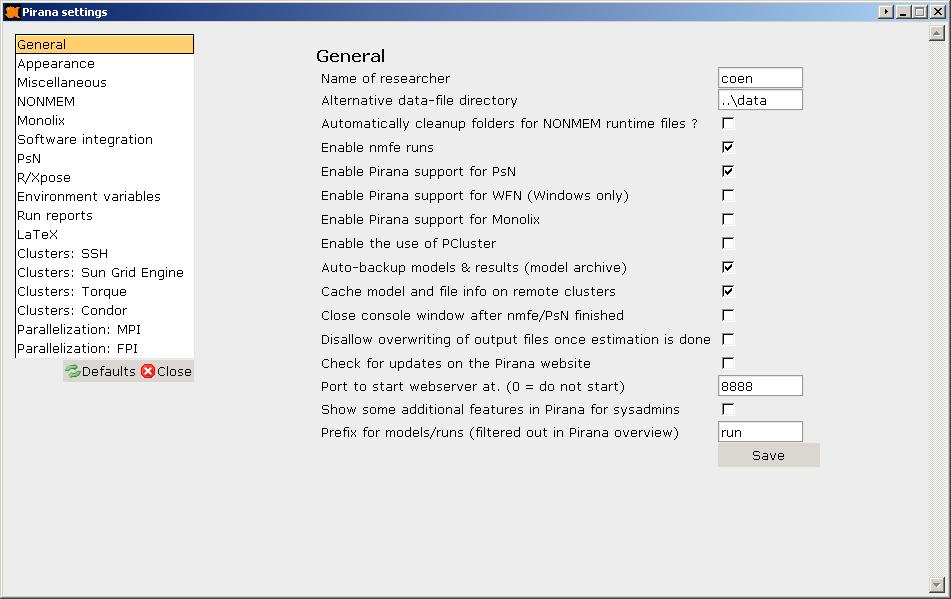
\includegraphics[scale=.4]{images/settings_1.jpg}
    \caption{General settings window}
\end{figure}

\subsubsection*{NONMEM}
\begin{itemize}
\item Refer to the NONMEM quick guide for detailed support on how to setup NONMEM instatllations. 
\item This is not necessery if PsN is used. 
\end{itemize}

\subsubsection*{Software integration}
\begin{itemize}
\item The software integration tab (Figure 2) deals with the integration of other software packages into Pirana. 
\item If the background of a software location appears green, the program can be found, whereas if it is red the program cannot be located under the specified path.
  \item Except for the list of programs defined below,  \emph{all other items in the software integration window are not necessery to define in order to work with Pirana}. Most other programs locations are only used to create easy links to the software from within Pirana. Also the location of \emph{psn.conf} is not needed to work with PsN.
 \item The following software packages are important to set correctly in order to work with Pirana easily: 
 \subitem \emph{R location}; Pirana uses R and Xpose to generate graphs, hence it is important to set the path to R correctly.
 \subitem \emph{Location of R GUI} (if available); if a GUI for R is available this should be specified. RStudio is recommended.
 \subitem\emph{ Spreadsheet location} (i.e. Excel, Numeric etc.), to view the contents of CSV files.
 \subitem\emph{ Code/text editor}; This editor will be used to edit models or scripts and is therefore important to define. 
 \subitem\emph{ PDF file viewer}; Many graphics are created as PDF files, hence a PDF viewer is useful to define.
\end{itemize}
%% Fig 2
\begin{figure}[h] \centering
    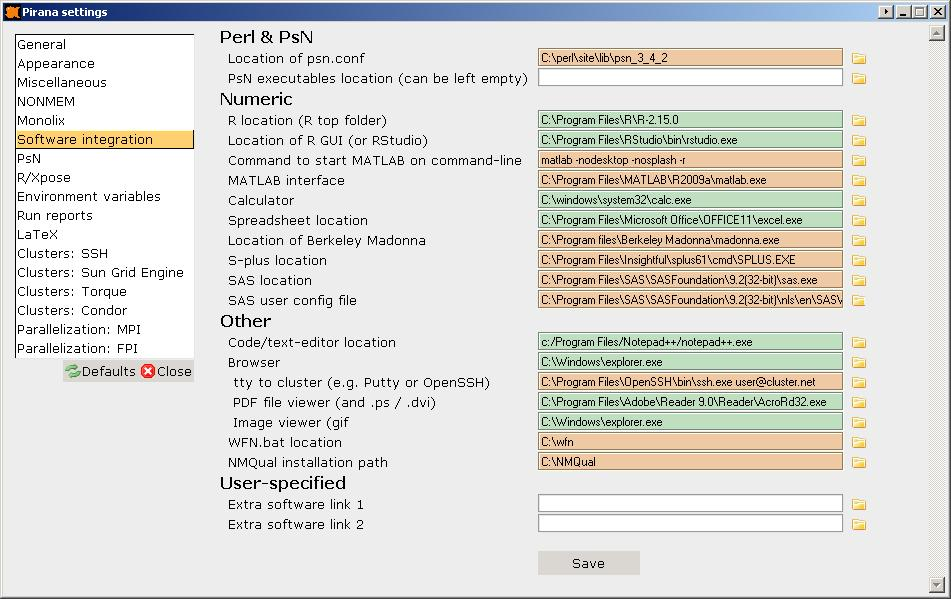
\includegraphics[scale=.4]{images/settings_2.jpg}
    \caption{Software integration window}
\end{figure}

\subsubsection*{PsN}
\begin{itemize}
\item Refer to PsN quick guide for detailed support on using PsN with Pirana.
\item This settings window specified default command line parameters for PsN.
\end{itemize}

%% Fig 3
\begin{figure}[h] \centering
    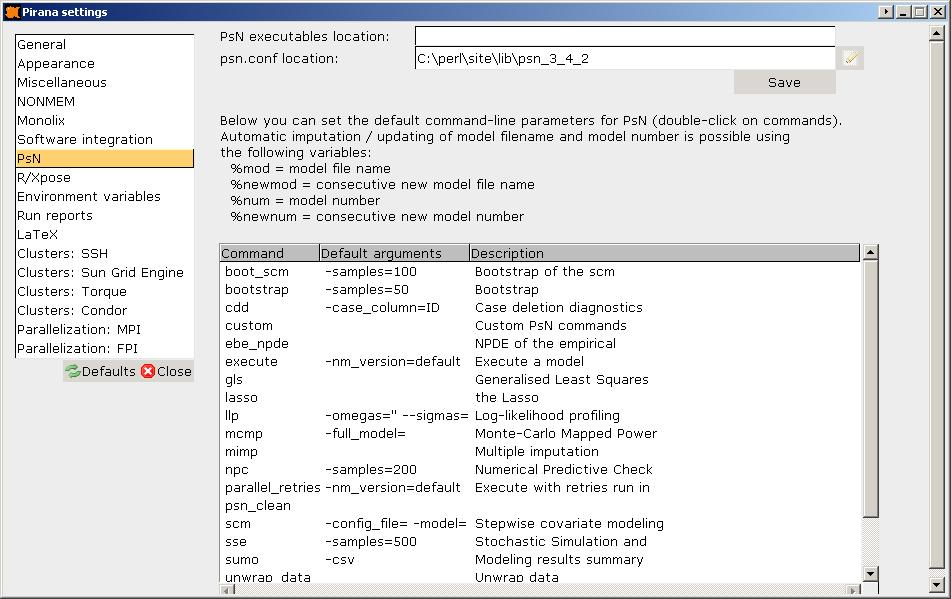
\includegraphics[scale=.4]{images/settings_3.jpg}
    \caption{PsN settings window}
\end{figure}

\subsubsection*{R/Xpose}
\begin{itemize}
\item \emph{Initialization commands} may be used to load specific R libraries when executing R/Xpose. 
\item \emph{PDF/PNG/GIF/EPS Arguments}: Default plotting arguments for R printing devices.
\item \emph{Sweave preamble/postamble}: If the Sweave functionality from Xpose is used, the default LaTeX pre/postable may be specified here.
\end{itemize}

%% Fig 4 
\begin{figure}[h] \centering
    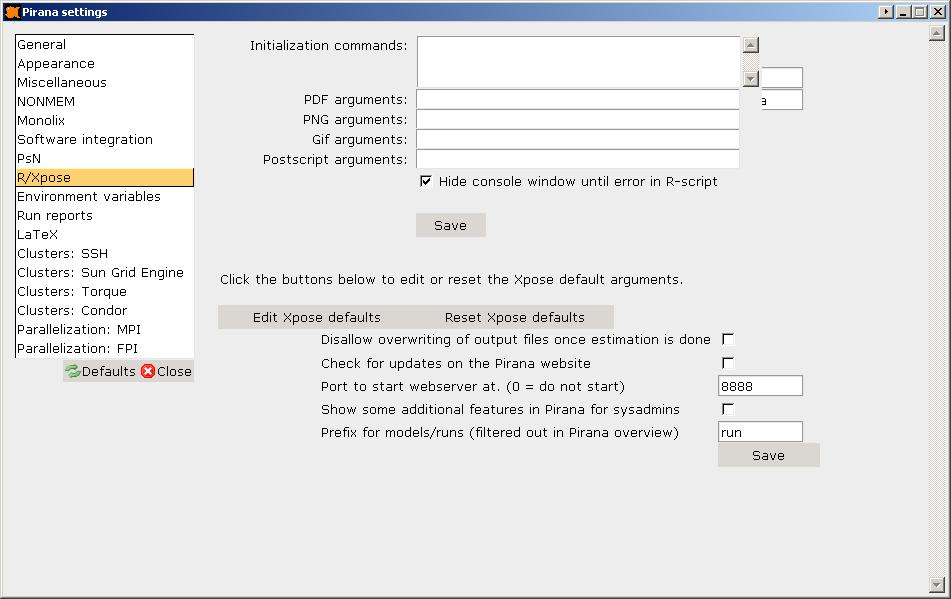
\includegraphics[scale=.4]{images/settings_4.jpg}
    \caption{R/Xpose settings window}
\end{figure}

\subsubsection*{Clusters}
\begin{itemize}
\item For more information on settings for clusters, please refer to the Clusters quick guide.
\end{itemize}

\subsubsection*{Configure the Sun Grid Engine}
\begin{itemize}
\item Defaults for working with SGE may be defined here.
\end{itemize}

%% Fig 5
\begin{figure}[h] \centering
    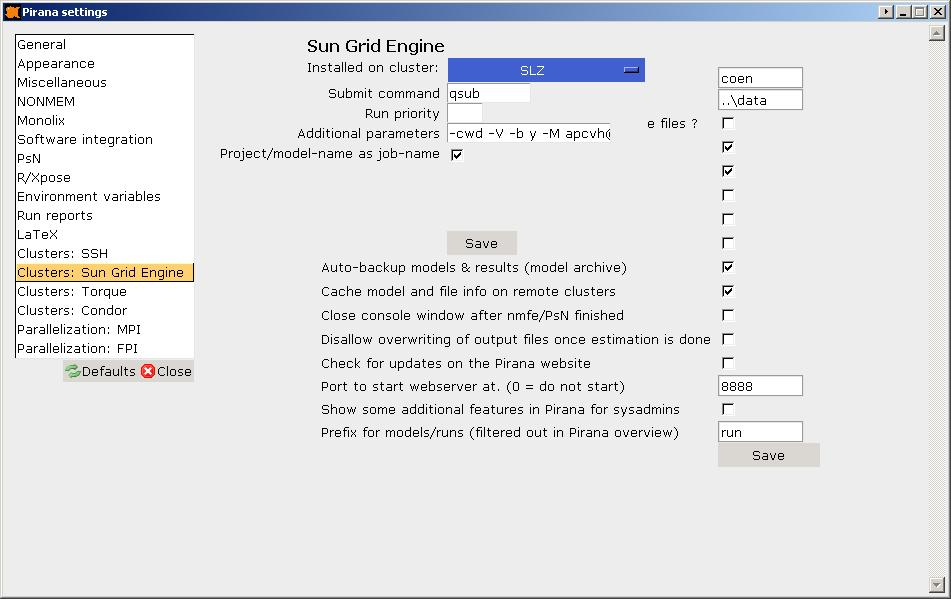
\includegraphics[scale=.4]{images/settings_5.jpg}
    \caption{SGE}
\end{figure}

\subsubsection*{Miscellaneous}
\begin{itemize}
\item \emph{File extensions}: File extensions are important to define because this wil determine if model files are shown (i.e. mod or ctl), and if NONMEM output files are correctly read (i.e. res or lst). 
\item \emph{Linux}: Refers to defaults for terminal and shell
\item \emph{PCluster}: Settings for working with PCluster (unsupported, refer to PCluster manual).
\item \emph{NMQual settings}: Here, folders may be added to PATH or LIBRARY\_PATH environmental variables.
\end{itemize}

%% Fig 6
\begin{figure}[h] \centering
    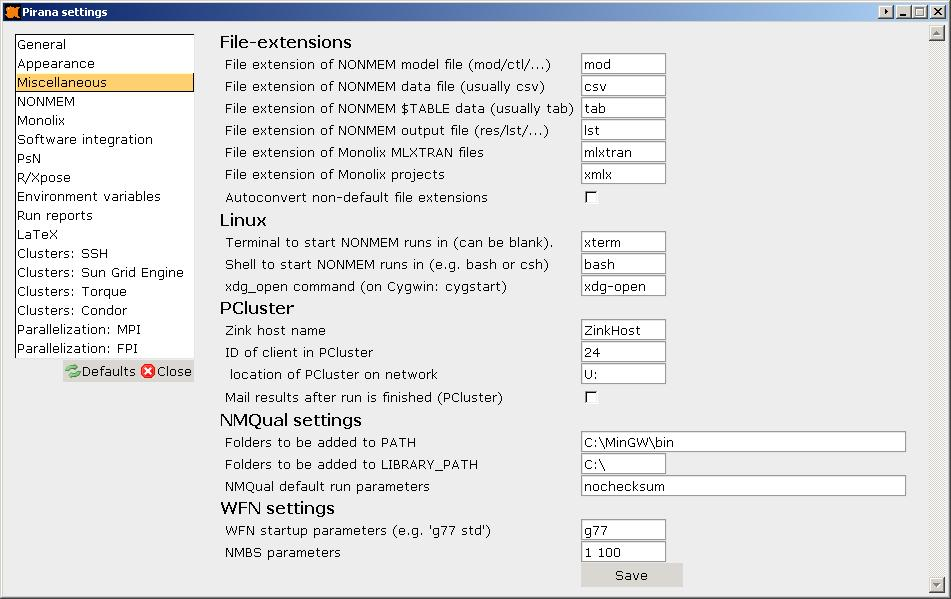
\includegraphics[scale=.4]{images/settings_6.jpg}
    \caption{Miscellaneuous settings}
\end{figure}

\end{document}

